\chapter{Resultados}
\label{cap_results}

Nesta secção será realizado um estudo sobre os resultados e competências da solução implementada.

Como discutido previamente, a solução desta tese é composta por 3 módulos distintos, cada um deles tendo sido explorado em capítulos dedicados, mas dos quais 2 - OSDOCR Pipeline e OSDOCR Editor - são dependentes e produtos do 1º, sendo este, OSDOCR Toolkit, a base do projeto como um todo.

Desta forma, será dedicada uma secção para cada uma destas componentes, com especial tratamento para a primeira pois, sendo um caso particular de implementação que dificulta uma apreciação sucinta, pode ser tomada como seus resultados, os próprios resultados das outras duas componentes.

As duas restantes componentes terão também por sua vez métricas de apreciação distintas, que serão nas respetivas secções explicadas.


\section{OSDOCR Toolkit}


O toolkit para melhoria do processo de OCR serviu como objetivo base do atual trabalho. Este, através do estudo do estado da arte, reflexão sobre a filosofia da solução, assim como pelo cíclico processo de implementação e teste, evoluiu para englobar diferentes aspetos da aplicação de OCR: desde o processamento de imagem; tratamento, análise e manipulação dos resultados de OCR; e tratamento de texto.
Dentro destes foi evidente o foco na segunda componente do processo, sendo a que menor atenção tem nas soluções correntes, que tendem a focar no processamento de imagem ou tratamento de texto fazendo uso de deep learning.

Existem diferentes formas de avaliar um toolkit, como: a apreciação da capacidade das suas ferramentas de forma individual; a sua utilidade em contextos além dos designados para a sua utilização; e a capacidade de integração em soluções mais complexas, i.e. soluções que façam uso do toolkit.

Ao longo do capítulo \ref{cap_osdocr_toolkit_implementacao}, à medida que eram expostas as diferentes ferramentas desenvolvidas, exemplos do uso destas foram sido fornecidos, estando uma demonstração individual destas já fornecido.

A solução engloba ainda 2 outras componentes que, como base, fazem uso deste mesmo toolkit. Estas 2 componentes, ambas também com o foco concreto de uso em jornais antigos, podem ser utilizadas em contextos extra, como revistas ou documentos atuais. Assim, através da avaliação destas 2 soluções, podemos simultaneamente, embora indiretamente, avaliar o Toolkit.

% dificil de verificar resultados devido a metodos nao produzirem diretamente resultados

% verificar aplicacao de alguns metodos especificos

\section{OSDOCR Pipeline}


A pipeline de aplicação de OCR é, das 3 componentes da solução, a que mais facilmente pode ser objetivamente discutida. Esta é das 3 a que se assemelha mais aos trabalhos envolvendo aplicação de OCR, onde se tem um resultado direto e comparável com um valor inicial, i.e. texto real de um documento (ground truth), do qual se podem obter diferentes métricas, comparado com o texto resultante da aplicação de OCR numa imagem.

Seguindo um processo semelhante, obter-se-ão então resultados da aplicação desta componente sob diferentes casos de teste. 

Relativamente aos casos de teste escolhidos, estes constam um total de 18 diferentes jornais, para um total de 35 páginas a serem testadas. O número amostras é inferior ao ideal sendo limitado pelo escopo do projeto - com uma solução envolvendo 3 componentes, todas de considerável dimensão -; à necessidade de, na generalidade dos casos, ser necessária uma cuidada e manual transcrição das amostras escolhidas; e múltiplas utilizações de cada amostra para diferentes resultados.

As amostras escolhidas apresentam, de modo a testar diferentes capacidades da pipeline, características particulares que as permitem caracterizar em :

\begin{itemize}\setlength\itemsep{-0.9em}
	\item \textbf{Template compacto (4)} : templates com muito texto, compactado, e normalmente resolução abaixo da desejada; 
	\item \textbf{Ordem de leitura complexa (2)} : templates que apresentam uma ordem de leitura não linear (cima para baixo, esquerda para a direita), fazendo uso do contexto do texto ou de guias (ex.: delimitadores) para guiar o leitor;
	\item \textbf{Moderno (1)} : jornais modernos, com resolução e estado ideal;
	\item \textbf{Inclinados (2)} : jornais que foram digitalizados com má orientação;
	\item \textbf{Template simples (4)} : Jornais que apresentam um template e, consequentemente, uma ordem de leitura simples. Texto/colunas bem espaçados;
	\item \textbf{Outros (5)} : outros tipos de documentos como: revistas, jornais infantis com muitas ilustrações, banda desenhada, etc.;
\end{itemize}

Para cada um destes documentos, uma transcrição foi preparada manualmente, assim como ficheiros adicionais com transcrição parcial, e com características do documento como o número de artigos, imagens e colunas. 
Tal deve-se á escolha do módulo de validação da pipeline para obtenção e comparação de resultados. Este, como descrito na secção correspondente, procura comparar através de diferentes métricas uma verdade de um documento (ground truth) com os resultados obtidos de diferentes configurações da pipeline.

As métricas que nos focaremos para a tabulação de resultados serão:

\begin{itemize}\setlength\itemsep{-0.9em}
	\item Variação da confiança de texto
	\item Similaridade do texto (similaridade de coseno)
	\item Comparação entre aparições de palavras na GT e no resultado
	\item Comparação entre palavras únicas na GT e no resultado
	\item Presença dos excertos da GT parcial no resultado
	\item Ordem dos excertos da GT parcial no resultado
	\item Ordem geral final no resultado \footnote{* - manualmente analisada}
	\item Número de artigos encontrados
\end{itemize}


\begin{figure}[H]
	\centering
	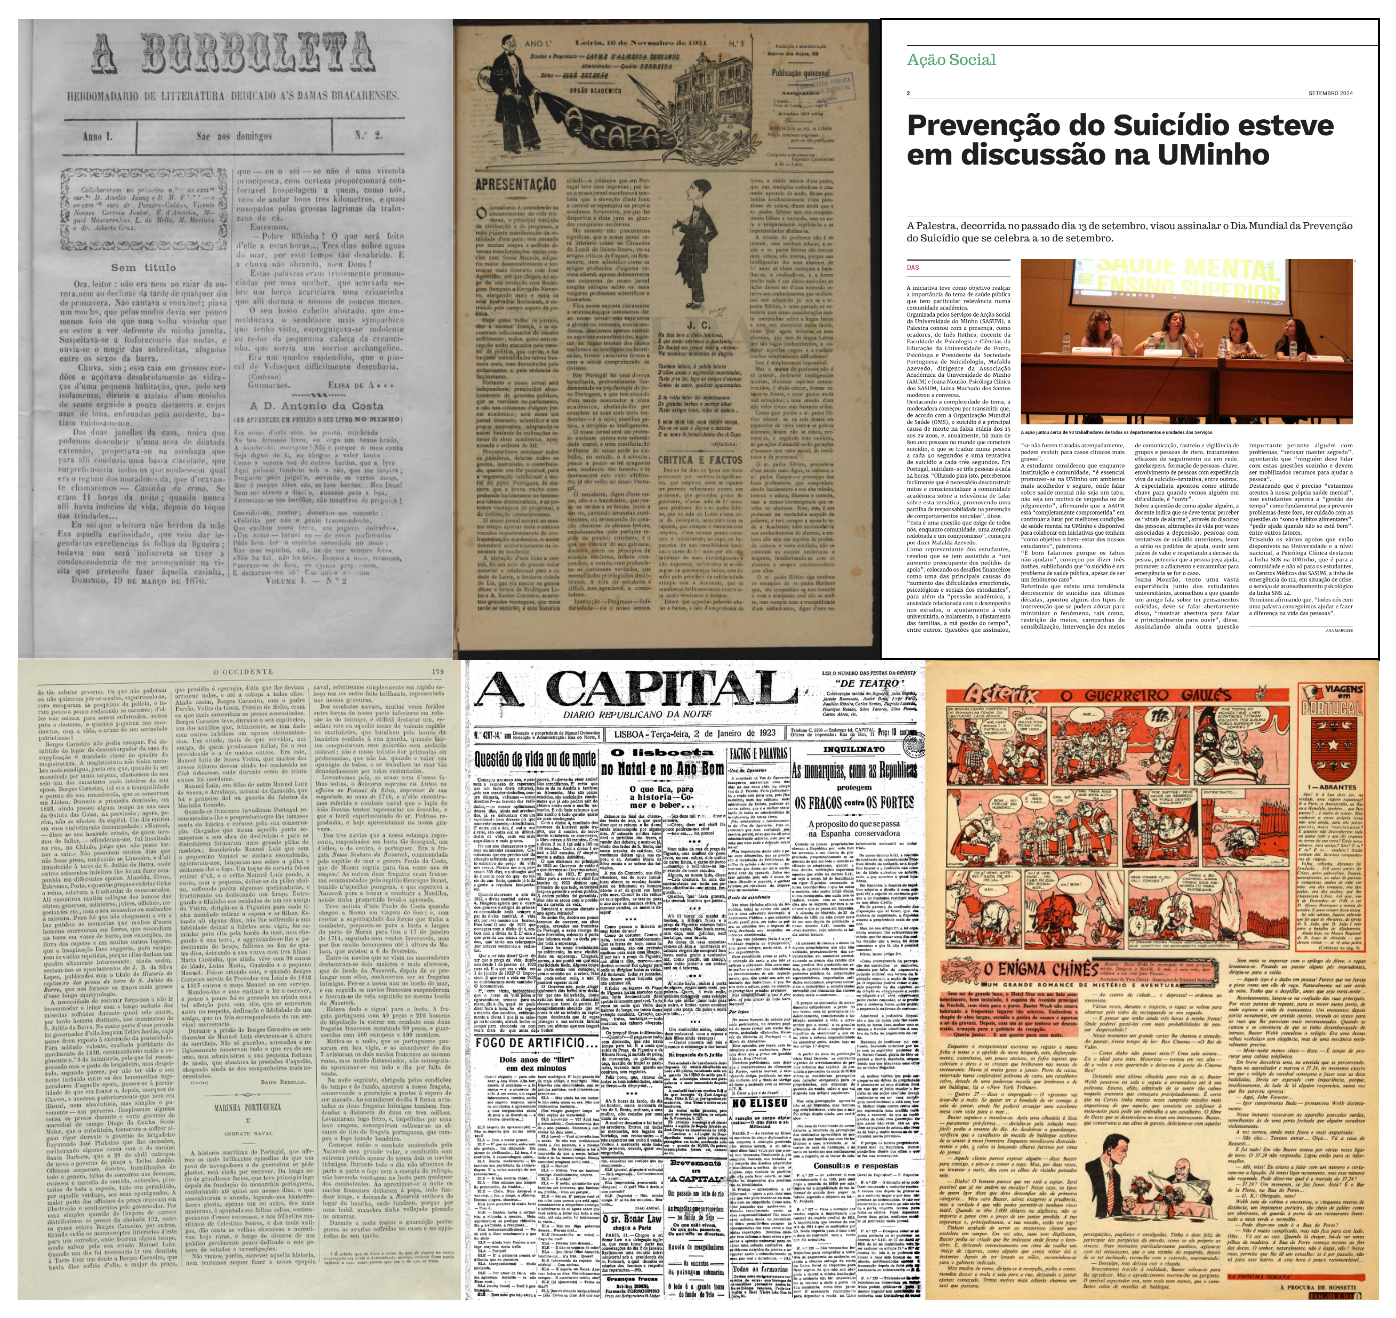
\includegraphics[width=0.7\textwidth]{images/ilustracoes/casos_teste.png}
	\caption{Amostras do conjunto de casos de teste.}
	\label{fig:casos_teste}
\end{figure}


Sendo a pipeline mutável através da configuração a ela passada, diferentes configurações foram desenhadas para possibilitar a extrapolação de mais conclusões. Note-se que esta lista não é extensiva, sendo que estas são multiplicativas ao número de execuções total.

Como base, será usada uma configuração de pipeline que não fará uso de nenhum módulo desta para além de OCR.

As outras configurações são, de forma sucinta:

\begin{enumerate}\setlength\itemsep{-0.9em}
	\item Pipeline completa: utilizada para testar uma sequência de todos os módulos implementados.
	\item Pipeline completa sem ordenação: possibilitando a comparação da ordenação original com a aplicação dos módulos.
	\item Apenas pré-processamento: permitindo a avaliação dos módulos de imagem na transcrição
	\item Apenas pós-processamento: afetando principalmente a capacidade de melhorar a leitura da transcrição geral
	\item Pipeline geral: configuração que, ao longo do trabalho, se avaliou como sendo mais ubíquo (relativamente)
\end{enumerate}

Como características gémeas entre estas configurações, temos que todas utilizam o tesseract como motor de OCR, utilizando a configuração de linguagem 'por' para português visto ser esta a linguagem dos casos de teste. No caso de ser realizado upscaling da imagem, procura-se aumentar os dpi para 150, assumindo uma dimensão de folha A3, ocorrendo para a generalidade dos casos o upscaling (exceção a categoria moderna).

No total, serão analisadas 210 (6 configurações x 35 páginas) execuções da pipeline.



Todos os preparativos para esta análise (jornais, ground truths e configurações de pipeline), assim como os resultados pré tabulados, estão disponíveis \href{https://drive.google.com/drive/u/0/folders/1DW-AIuSxjEyv6ioq7jX8P1xruy03Sxo9}{aqui}.

% aplicacao da pipeline nos casos de estudo
%% realcar situacoes particulares de sucesso ou de problemas


\section{OSDOCR Editor}


A última componente a analisar é o editor. Este tem como base o Toolkit e, como \textit{modus operandis}, a manipulação da estrutura OCR Tree. 

A sua proposta principal, como discutido nas proposições do capítulo \ref{cap_osdocr_filosofia}, é a disponibilização de um ambiente gráfico para fácil manipulação da estrutura de dados universal OCR Tree, consequentemente permitindo fazer reparos minuciosos nos resultados da pipeline e, servir como uma poderosa ferramenta de debugging da pipeline e do toolkit.

Através das suas funcionalidades, além da persistente dependência no Toolkit, também faz uso da pipeline - como é exemplo a aplicação de OCR localmente, ou reutilização do módulo de extração de output -, sendo portanto relevante como parcial resultado destes, especialmente do toolkit.

Como o toolkit, a avaliação desta componente não é direta, a não ser num cenário de extensa listagem das funcionalidades, isolados e combinadas, analisadas em diferentes casos de utilização. Alguns destes já foram descritos para funcionalidades mais relevantes e únicas desta componente, no seu capítulo de implementação. 

Outra forma de avaliar esta ferramenta, mais subjetiva embora não menos relevante, provém do uso de grupos de utilizadores. A estes poderiam ser dados conjuntos de tarefas a realizar, e registadas as dificuldades (ou falta delas) na sua execução, opiniões sobre as capacidades da ferramenta, e capacidade de as executar sem apoio externo. Esta metodologia não foi seguida, por restrições de tempo, mas é importante realçar a sua relevância no contexto de disponibilização da ferramenta para um público mais amplo, assim como a sua acessibilidade para sujeitos menos envolvidos no contexto técnico.

A avaliação seguida baseia-se então na apresentação das capacidades e adaptabilidade desta interface gráfica, através da listagem de casos de uso distintos e contrastantes.


\begin{itemize}\setlength\itemsep{-0.5em}
	\item Análise e manipulação de ficheiros do tipo OCR Tree, i.e. formato json e hocr : aplicabilidade para resultados de soluções além da OSDOCR pipeline.
	
	\item Visualização de diferentes níveis da OCR Tree.
	
	\item Filtragem da OCR Tree: através de filtros de tipo, texto, coordenadas e ID.
	
	\item Fácil retrocesso e reconstrução de operações complexas sob a OCR Tree: através de uma cache de OCR Tree.
	
	\item Limpeza de blocos de ruído de OCR Tree.
	
	\item Ajuste de dimensões e posicionamento de blocos da OCR Tree.
	
	\item Divisão de blocos através da ferramenta de corte : sem GUI seria necessário manualmente modificar as árvores, respetivamente atualizando o texto dos filhos e as suas coordenadas.
	
	\item Junção facilitada de blocos : sem GUI seria necessário modificar as árvores, mantendo apenas uma modificando as suas coordenadas e, especialmente, realocando os filhos de acordo com o seu posicionamento. Especialmente difícil na junção de árvores com texto que se intercala ou sobrepõe.
	
	\item (Re)categorização de blocos.
	
	\item Modificação direta do texto de blocos : manualmente seria necessário modificar as folhas para atualizar ou adicionar palavras, e criar novos nodos para cada linha e parágrafo.
	
	\item Criação de blocos não existentes.
	
	\item Realizar OCR num bloco : servindo para melhorar texto e a sua confiança por transcrição máquina.
	
	\item Realizar OCR num segmento da imagem: gera, de acordo com a segmentação do motor OCR, múltiplos blocos com uma só ferramenta.
	\item (Re)ordenar blocos através da modificação do seu ID: modificação direta ou com ferramentas do Toolkit.
	
	\item Gerar OCR Tree numa imagem sem resultados.
	\item Visualizar resultados da OSDOCR Pipeline: útil para contexto de debugging e desenvolvimento.
	
	\item Corrigir resultados da OSDOCR Pipeline: sendo que este durante as vários módulos produz uma OCR Tree, pode-se corrigir um ponto específico.
	\item Visualizar resultados do OSDOCR Toolkit.
	
	\item Conversão de  OCR Tree em output textual simples.
	
	\item Conversão de OCR Tree em output textual de artigos.
	
	\item Segmentação da OCR Tree em artigos : manual ou utilizando métodos do toolkit.
	
	\item Manipulação de artigos : reordenação, atualização, inserção e remoção.
	
	\item Criação de OCR Tree para segmento de uma imagem com respetiva OCR Tree : com input de imagem e OCR Tree, a ferramenta de divisão de imagem gera uma nova imagem, partição da primeira, com uma OCR Tree constando cópias dos blocos que estavam inseridos e/ou intersetados (dependo das configurações do editor) na partição. Facilita assim a criação de resultados de OCR para partição de uma imagem que já possui resultados.
	
	\item Criação facilitada de resultados de confiança para jornais antigos manualmente: como intendido pela premissa da tese.
	
	\item Criação de resultados de confiança para documentos de outro tipo manualmente: não sendo tão focado para documentos que produzam resultados ruidosos, amplia a utilidade da solução; ex. documentos aplicáveis: banda desenhada, livros, revistas, recibos, etc..
	
	\item Suavização do processo de criação de ilustrações no contexto de OCR e manipulação da OCR Tree: como prova deste conceito, tem-se que a maioria das imagens desta dissertação fizeram uso do OSDOCR Editor
\end{itemize}

